\documentclass{theme/franska}
\documentclass[a4paper,margin=3.25cm]{article}
%\documentclass[a4paper,margin=3.25cm]{article}
%[a4paper,margin=3.25cm]{geometry}


% Filler text
\usepackage{lipsum}
\usepackage{verbatim}
% Footer and header
\usepackage{fancyhdr}

%\setcounter{secnumdepth}{4} % how many sectioning levels to assign numbers to
%\setcounter{tocdepth}{4}    % how many sectioning levels to show in ToC


% Allow bilagor
\usepackage{standalone}

%nice tablesVälkomna till teaterföreställningen Alice i underlandet. Kom och se eleverna i estetisk kommunikation framöra sin originella version av Lewis Carolls berättelse om Alice. Det blir en resa med alla sinnen: syn, hösel, känsel och smak!
\usepackage{booktabs}
\renewcommand{\arraystretch}{1.2}


%bibliography packages
\usepackage[sorting=ynt]{biblatex}
\addbibresource{sample.bib}
\usepackage[nottoc]{tocbibind}

% Language package
\usepackage[utf8]{inputenc}
\usepackage[english,swedish]{babel}

%Quotations
\usepackage{csquotes}


%Images
\usepackage{graphicx}
\graphicspath{ {bilder/} }


\usepackage{fancyhdr}

% Header and footer
	\pagestyle{fancy}
	% Clear headers and footers
	\fancyhead{}
	\fancyfoot{}
	% Remove line in the header
	\renewcommand{\headrulewidth}{0pt}
	% Draft, header
	\fancyhead[C]{--- Utkast ---}
	% Pagenumber, footer
	\fancyfoot[C]{\thepage}
	% Git commit data, footer
%	\fancyfoot[R]{{\tiny Rev: \git}}

%\fancyhead{}
%\fancyhead[RO,LE]{Thesis Title}
%\fancyfoot{}
%\fancyfoot[LE,RO]{\thepage}
%\fancyfoot[LO,CE]{Chapter \thechapter}
%\fancyfoot[CO,RE]{Author Name}






\begin{document}

	% Set main language
	\selectlanguage{swedish}

	% Frontpage

	%Första sidan räknas inte
    \clearpage\thispagestyle{empty}\addtocounter{page}{-1}

	\begin{titlingpage}
\begin{SingleSpace}
\calccentering{\unitlength}
%\begin{adjustwidth*}{\unitlength}{-\unitlength}
\vspace*{13pt}
\begin{center}
\rule[0.5ex]{\linewidth}{2pt}\vspace*{-\baselineskip}\vspace*{3.2pt}
\rule[0.5ex]{\linewidth}{1pt}\\[\baselineskip]
{\HUGE Franska Skolan }\\[4mm]
{\Large \textit{Gymnasie Arbete}}\\
\rule[0.5ex]{\linewidth}{1pt}\vspace*{-\baselineskip}\vspace{3.2pt}
\rule[0.5ex]{\linewidth}{2pt}\\
\vspace{6.5mm}
{\large Av}\\
\vspace{6.5mm}
{\large\textsc{Getz Mikalsen}}\\
\vspace{11mm}

\includegraphics[scale=0.6]{logo}\\
\vspace{6mm}
{\large Gymnasie Arbete\\
\textsc{Franska skolan}}\\
\vspace{11mm}
\begin{minipage}{10cm}
%%DUMMY TEXT HERE
\lipsum[66]
%%DUMMY TEXT ENDS HERE
\end{minipage}\\
\vspace{9mm}
\today        %%Date of compilation
%%{\large\textsc{Oktober 2014}}  Other date
\vspace{12mm}
\end{center}
%\begin{flushright}
%{\small Antal ord: \wordcount}
%\end{flushright}
%\end{adjustwidth*}
\end{SingleSpace}

\end{titlingpage}

\pagebreak




	% Select English as language before the Abstract
	\selectlanguage{english}
	\begin{abstract}

Nutmeg is an easily obtainable spice and has been widely used for centuries because of its seasoning effect but also because of its psychotropic properties.
The active ingredients in nutmeg is thought to be resididing in the volatie oil, where myristicin, elemicin and safrol are thought to be the primary components involved in the intoxicative syndrome.

Today's report is divided into three separate portions.
A history of nutmeg and the extent of its usage in various cultures is presented, a brief introduction of the history of nutmeg is also presented.

The remainding two portions of the report will be divided into separate parts. The discussion of nutmeg and its composition, and the possible involvement of its chemical components and their amine derivates.

The first is a description of the plant and its composition; followed by a presentation of the suggested measures for isolating and identifying the many components in the oil from the plant. This is followed by a definition of those components thought to be involved in the intoxicative syndrome.

The extension of these components to their respective amphetamines, and their effectiveness in humans, and the possibility of them being an acceptable explanation to the intoxicative syndrome of nutmeg, will constitute the latter part of this report.


% Our report today has been divided into two separate portions. The discussion of nutmeg and its composition, and of the possible involvement of its chemical components. The psychotropic intoxication has a natural division into two areas of presentation. The first is a brief description of the plant; a presentation of the methods and procedures for the isolation and the identification of the many components in the oil from the plant, and a careful definition of those components that are most probably involved in the intoxicative syndrome.

% The extension of these components in to the corresponding amphetami-nes, their effectiveness in humans, and the likelihood of their being an acceptable explanation of the effects of the total nutmeg, will constitute the latter part of this report. The introduction of this report will present some of the history of nutmeg, and a description of the style and extent of its usage in various cultures. In the reports that may follow, specific descriptions of the human syndrome of intoxication, and some of the pharmacological ramifications of its study, will be presented.

	\end{abstract}

	\begin{flushleft}
		{\small {\bf Keywords:} Nutmeg, Hallucinogen, Amphetamine, Phenetylamine, Volatile oil}
	\end{flushleft}

	% Return to Swedish as language
	\selectlanguage{swedish}

	\tableofcontents

	\clearpage

	\section{Introduktion}
	\subsection{Syfte}
%[Jag tror första 2 styckena av syftet passar mer som abstract fast på engleska]
%Denna rapport är delad i två delar. Diskussionen av muskotnöt samt dess innehåll, och den möjliga påverkan dess kemiska innehåll har.
%Den psykotropiska berusningen (intoxikationen??) kommer bli uppdelad i två områden i sin presentation. Den första är en beskrivning av plantan; en presentation av metoderna och procedurerna för isolering och identifikation av innehållet från plantans olja, och en noggrann förklaring av de beståndsdelar som mest troligt är involverade i det intoxikativa syndromet (kan man säga så? (intoxicative syndrome))

%Utsträckningen av dessa beståndsdelar till dess motsvarande amfetaminer, dess effektivitet i människor, samt dess sannolikhet att vara en godtagbar förklaring av effekterna av muskotnöt, kommer utgöra den senare delen av detta arbete. Det kommer även finnas en del som tar upp muskotnötens historia i början av arbetet, samt en beskrivning samt utsträckning av dess användande i diverse kulturer.

Jag att presentera en saklig beskrivning av de diverse ämnen som har funnits till att utgöra den flyktiga (och den förmodade aktiva \cite{shulgin1967chemistry}) fraktionen av muskotnöt. Hypotesen lyder så att en eller flera beståndsdelar av muskotnöten är tilldelad rollen för de berusande effekterna av muskotnöt. Därför behövs en exakt kemisk definition av muskotnöten. Men före detta, så måste vi definiera just vad som namnet muskotnöt betyder i botaniska termer.










%Syftet för denna rapport är att visa och förklara de psykoaktiva effekterna hos muskotnöt samt dess användningsområden utöver användningen som en krydda som återfinns i många svenska hem.
%Rapporten kommer att göra en uppställning av de eteriska oljorna i muskotnöt för att sedan göra en analys av de olika oljorna för att finna samband till andra kända psykoaktiva substanser.

	\subsection{Bakgrund}
Muskotnöt, kommer ifrån trädet \textit{Myristica fragrans}, som ursprungligen är ifrån de Indonesiska Bandaöarna (även känt som kryddöarna). Legenden har det att när \textit{M. fragrans} blommar så får den överväldigande doften av nötterna fåglarna att falla till marken. \cite{kreig1965green}
Detta kan ha mer att göra med de narkotiska egenskaperna av muskotnöten än dess doft.

Trots att invånarna av Bandaöarna inte använde muskotnötterna som en krydda så finns det underlag på att det använts som en medicin och krydda i Indien och i Mellanöstern så tidigt som 700 f.v.t., \cite{kalbhen1971nutmeg}, dess terapeutiska användningsområden har uppmärksammats av Arabiska läkare sedan 700-talet. \cite{weil1967nutmeg} Muskotnöt anlände inte i Europa förens Medeltiden och det finns motstridande källor på om det var Arabiska handelmän eller återvändande korstågsriddare som tog med sig kryddan till Europa. Muskotnöt var något av en exotisk handelsvara förens 1600-talet då Portugiserna upptäckte Bandaöarna.

Efter denna upptäckt förlorade muskotnöten dess status som exotisk handelsvara. På höjden av dess värde, bars muskotnöt av Européer som ett tecken på rikedom.

\subsubsection{Muskotnöt som krydda}
Den välkända nötens vanligaste användningsområde är som en krydda. Muskotnöten producerar även en krydda känd som muskotblomma, vilket är det brungula mjuka hölje som omger kärnan. Muskotblomma är en vanlig krydda i äldre svenska recept, och fortfarande i många norska. Den är något lenare i smaken är muskotnöt men båda används på liknande sätt i matlagning. Muskotblomma innehåller samma oljor som gör muskotnöten psykoaktiv. \cite{entheogenreview}

De två kryddorna var som populärast på 1700-talet i England, där de användes som krydda till många olika rätter, som
roast mutton, stewed pork, pies, puddings, and cordials. Muskotnöt samt muskotblomma
har även använts för att krydda mång andra rätter, som soups, gravies, milk products, fruit juices,
sweet sauces, gelatins, alcoholic beverages, snack foods, and breakfast cereals; [källa här eller?]
Trots Muskotnötens tidigare utbredda användning inom matlagningen och dess plats i de flesta kryddskåp så har dess användning förminskats till enstaka kryddning av pajer, kakor samt av äggtoddy. \cite{entheogenreview}


\subsubsection{Muskotnöt som medicin}
Sedan samma tid som muskotnöten blev populär som krydda så har den även
varit använd som med medicin.
Muskotnöten har använts för helande (medicinska?) syften runtom i världen,
sedan den introducerades till Europa och västvärlden så har
dess medicinska användningsområden att användts av Europeiska doktorer.
Trots att muskotnöten användes för väldigt många olika syften inom sjukvården
så finns det ett antal som är mer
värdiga att nämnas på grund av dess utbredda användning.

Nutmeg has been used to treat rheumatism in Indonesia, Malaysia, England, and China. The
essential oil is used externally to treat rheumatic pains, limb pains, general aches, and
inflammation. In England, far into the twentieth century, a nutmeg was simply carried in one's
pocket to ward off the pains of rheumatism (Rudgley 1998).


Nutmeg has been used for its sedative effect to treat nervous complaints and to promote sleep
in Malaysia and India. The inhabitants of the Moluccas would mix nutmeg with milk or a banana
drink to give to children as a sleep aid (Rätsch 2005). In Europe, older women would carry
nutmegs with them in silver graters to promote sound sleep (Krieg 1964). Nutmeg has also
been widely used as an analgesic.


Nutmeg is probably most widely used to treat stomach complaints. It has been used in South
East Asia, India, the Middle East, and Europe to treat stomach aches and cramps, to aid
digestion, and to dispel gas.


Perhaps the most infamous medical use of nutmeg, as mentioned earlier, is as an
abortifacient. It is not clear how far back this use dates, but it was a popular--albeit
ineffective-- “remedy” at the end of the nineteenth century and beginning of the twentieth
century.

While there doesn't appear to be any traditional use of nutmeg as a mood elevator, several
individuals have noted that it does indeed have such properties. The German writer Georg
Meister noted nutmeg's uplifting effects in his 1692 work Der Orientalisch-Indianische Kunst-
und Lust-Gärtner (Oriental-Indian Art and Pleasure Gardener) commenting that "it can greatly
refresh even the ill and cheer them up with fresh spirits" (Rätsch 2005); and the twelfth century
mystic Hildegard von Bingen had this to say:

\begin{displayquote}

When a human being eats nutmeg it opens his heart, and his sense is pure, and it
puts him in a good state of mind. Take nutmeg and (in the same amount) cinnamon
and some cloves and grind them up. And then, from this powder and some water,
make flour--and roll out some little tarts. Eat these often and it will lower the
bitterness of your heart and your mind and open your heart and your numbed
senses. It will make your spirit happy, purify and cleanse your mind, lower all bad
fluids in you, give your blood a good tonic, and make you strong (Rätsch & Müller-
Ebeling 2006).

Rätsch, C. and C. Müller-Ebeling 2006. Pagan Christmas: The Plants, Spirits, and Rituals at the Origins of
Yuletide. Inner Traditions.

\end{displayquote}

Nutmeg is still used in Arabic and Indian folk medicine today, but its use as an herbal remedy in
Europe is long forgotten. Use as a medicine never seems to have caught on in the United
States, with the exception of its use as an abortifacient in the nineteenth century.



\subsubsection{Muskotnöt som afrodisiakum}

Ett mindre känt användningsområde av Muskotnöten är som ett afrodisiakum, vilket på vardaglig svenska betyder
kärlekselixir.
I Indien så har Muskotnöten använts till curry maträtter men även tuggbuss för dess (stämnings höjande effekter?) (afrodisiska effekter?) \cite{ratsch2005encyclopedia}

Medan användningen av Muskotnöten som ett afrodisiakum i Europa inte verkar vara något välkänte eller utbrett så
finns det enstaka exempel. William Salmon, en 1600-tals Engelsman skrev 1693, i ett själv-exeperiment där
Muskotnötsolja gnuggat på könet producerat sexuell lust (Sexual excitation) \cite{RudgleyR}.
Mest nämnvärt är nog en gammal Tysk folk tradition, där en flicka ska svälja en hel muskotnöt, samla den hela nöten
efter passage, göra den till ett puder och ha i maten av dess älskade. Att göra detta ska enligt traditionen
få mannen i fråga att förälska sig i flickan. \cite{ratsch2005encyclopedia}

Finns en studie där de använt råttor som test subjekt kan ta med den om jag orkar.


\subsubsection{Muskotnöt som dröm förbättrare}

Det finns inte mycket underlag angående hur muskotnöt samspelar med drömmar. Många experiment har beskrivit effekterna
av muskotnöt till dröm liknande kvalitéer och levande dagdrömmar. \cite{entheogenreview}
(Bilagor här www.erowid.com)

Den mest kompletta rapporten angående muskot nötens effekter på drömmar kommer ifrån Paul Devereaux, han intog
två teskedar av riven muskot och strödde ut den essentiella oljan av muskot på sin kudde samt lakan i en del
av ett själv experiment. Devereaux rapporterade att han blev helt självmedveten under drömmen där han flög igenom
en tunnel i en hög hastighet. Devereaux fann även att sina taktila sinnen var delvis funktionella i drömmen.
Devereaux beskrev hur han ryckte till sig löv från träd han passerade och även kände motkraften från grenarna samt
bladverket som grävde ner sig i hans hand. \cite{RudgleyR}

Devereauxs rapport stärker påståendet att muskot kan ha en effekt på klarheten av drömmar samt dröm återkallning,
likväl, mer definitivt underlag för dessa påståenden saknas.


\subsubsection{Muskotnöt som berusningsmedel}

Historisk sett har Muskotnöt använts i Egypten som ett surrogat för hashish. Det har även används i Indien, antingen
tuggat, eller snusat tillsammans med tobak, eller med tuggtobak, men det finns lite information kring dessa
administreringsvägar.

Muskotnöt introducerades först som en krydda i Europa och senare som en medicin. Europeerna
fortsatte dock att ignorera denna populära kryddas berusande effekter i flera århundranden.

Den första dokumenterade fallet av muskotnöt som ett berusningsmedel finner vi år 1576 när en
gravid brittisk kvinna drabbades av yrsel efter hon intagit mellan tio och tolv muskotnötter. \cite{stein2001nutmeg}

Skulle det inte varit för ryktet av muskotnötens effektivitet som ett abortmedel så skulle dess
psykoaktiva egenskaper troligtvis förblivit okända för en lång tid.
Enskilda fall av muskotnöts förgiftning var senare publicerade, men muskotnötens
berusande egenskaper förblev mestadels obemärkta och outforskade.

I det sena 1800-talet och tidigare 1900-talet så blev muskotnöten återigen populär som ett
abortmedel. I och med detta ökade fallen av muskotnöts förgiftning och fler fallstudier rapporterades.
Detta hjälpte till att måla en klar bild av muskotnötens verkan och effekter.
Det är inte säkert hur muskotnöten kom till att bli en rekreations-drog, men det verkar ha sitt
ursprung i det tidiga 1900-talet när dess användning uppstod i USAs fängelsen som ett alternativ
till marijuana och andra otillåtna substanser.
Vissa författare tyder på att muskotnötens användning som narkotika inte uppstod förens efter
andra världskriget. Dock så rapporterar Malcolm X i sin autobiografi att det redan funnits en kultur kring
användandet av muskotnöt vid Charlestown state Prison år 1946, detta tyder på att fångarna redan
varit bekända med muskotnötens narkotiska effekter för en viss tid.
Malcolms X ord löd såhär i sin autobiografi, utgiven 1965:
\begin{displayquote}

I first got high in Charlestown on nutmeg. My cellmate was among at least a
hundred nutmeg men who, for money or cigarettes, bought from kitchen worker
inmates penny matchboxes full of stolen nutmeg. I grabbed a box as though it
were a pound of heavy drugs. Stirred into a glass of cold water, a penny
matchbox full of nutmeg had the kick of three or four reefers \cite{malcolmx}.

\end{displayquote}

Efter utgivandet av Malcolm X sin autobiografi så sprakades intresset av muskotnöt som ett
berusningsmedel återigen i liv och intresset har levt kvar tills nutid.
Användandet av muskotnöt i fängelsen blev så småningom så utbredd att muskotnöt blev
helt bortplockat ifrån fängelseköken.




\subsubsection{Effekter av Muskotnöt}

Psykologiska effekter av muskotnöt innefattar, torr mun, illamående, hjärtrusning, rodnad,
domnandet av lemmar, hypotension (lågt blodtryck), eufori, avskildhet, CNS-excitation,
hallucinationer samt andningssvårigheter.
Muskotnöt har ingen märkvärd effekt på storleken av pupiller. \cite{entheogenreview}

Muskotnöt är bäst beskriven som en deliriant. I låga doser delar den karaktären av en kombination av alkohol och marijuana. I högre doser är effekterna mer lika de hos tropana alkaloider, ex. scopolamine och orsakar förvirring, disorientation samt hallucinationer.
Effekterna av muskotnöt kommer och går i vågor. I ena stunden kan det vara en känsla av onykterhet och i andra stunden kan den känslan ha avtagit.
Som effekterna avtar så blir avgränsningen mellan en vanlig och en icke vanlig verklighet tunn och tillåter användaren att övergå mellan de två med någon form av kontroll.

En anledning till att effekterna av muskotnöt bibehåller sin mystik för många är att muskotnötens berusning följer en unik tids-linje. Detta är även möjligtvis anledningen till fientligheten som finns mot muskotnöt som ett berusningmedel. Många antar att muskotnöt kommer producera effekter som utvecklar sig inom en timme vilket de gör med de traditionella psykadeliska drogerna som psilocybin-innehållande svampar eller LSD. Vilket det inte gör, användaren tror att den inte tagit tillräckligt då den inte upplever några önskade effekter och ökar dosen. Detta leder till en oavsiktlig överdosering och en berusning utöver den först önskade. (För att bäst beskriva muskotnötens berusning och för att undvika missöden så har jag delat upp dem i olika steg och summerat effekterna som kan upplevas vid respektive steg.(tror jag hoppar detta, skriver kolla bilaga))

\\

%\paragraph{Inledande berusning (timmar 4-8)}


%\paragraph{Topp berusning (timmar 8-12)}


%\paragraph{Slut av topp (timmar 13-18)}


%\paragraph{Rest berusning (timmar 19-25)}


%\paragraph{Sista steget-baslinje (timmar 26-32)}


\subsubsection{Dosering av Muskotnöt}
Hur potent muskotnöten är kan variera kraftigt mellan en nöt och en annan;
man bör vara medveten om sitt stoff innan man intar en större dos.
Muskotnötter från Östindien sägs vara mer potent än de producerade i Västindien, och färskt
mald muskot är även känt att vara mer potent än för mald muskot.\cite{entheogenreview}
Muskotnöt är inte att utsättas till justeringar av dosering i efterhand pågrund
av dess sena utveckling av effekter, detta gör att en kännedom om potens viktig.
\cite{entheogenreview}

\\

Den följande informationen angående dosering är baserade på en analys av 176 erfarenheter publicerade online på Erowid.com

\paragraph{Tröskel (3-5 gram eller 1-1.5 tsk)}
En tröskel dos av muskotnöt utmärks av en eufori, avslappning, humörs höjning, glädje samt
förstärkning av sinnena.
Vissa personer upplever inga effekter vid denna nivå.

\paragraph{Låg-Måttlig (6-10 gram eller 1.5-3 tsk)}
En låg-måttlig dos av muskotnöt kan producera mer distinkta effekter än en tröskel dos, kan framkalla visuella förvrängningar, CEVs, samt hörselhallucinationer.
Korttidsminnet kan försämras och tal kan bli något sluddrigt under toppen av en
låg-måttlig dos.

\paragraph{Måttlig (11-15 gram eller 1-1.5 msk)}
En måttlig dos av muskotnöt kan orsaka sluddrigt tal, desorientering, och förlust av koordination. Tidigare nämnda effekter ökas och brukaren kan uppleva milda visuella fenomen.

\paragraph{Måttlig-Hög (16-20 gram eller 1.5-2 msk)}
En måttlig-hög dos kan producera ett vaket dröm likt tillstånd. En individ sökte intensiv vård efter ett intag av 15-20 gram av muskotnöt. Individen rapporterade andningssvårigheter, medvetslöshet, inbillningar samt panik.

\paragraph{Hög (20-25 gram eller 2-2.5 msk)}
En hög dos kan fortsatt förstärka inbillningen att användaren befinner sig i en dröm värld. Användare kan uppleva magont.

\paragraph{Icke rekommenderad (25+ gram eller 2.5+ msk)}
Doser vid denna grad ökar generellt sett inte de psykoaktiva effekterna av muskotnöt, men kommer mer troligt att öka tidsomspannet av intoxikationen (berusningen) och vill med det ta längre att återhämta sig från.
Fysiskt obehag som magont, hjärtklappningar, illamående samt yrsel tenderar att öka.
Kräkningar inträffar sällan.
Användaren kan uppleva andningssvårigheter eller svårheter med urinering. Användaren kan också få vanföreställningar.
Utav 66 individer som rapporterat ett intag av över 25 gram av muskot, 17\% rapporterade en svår upplevelse och 45\% av dom uppsökte akut-sjukvård.
Den genomsnittliga dosen för de som rapporterade negativa effekter var mellan 29 och 30 gram, dock var median dosen endast 25 gram. Genomsnittsdosen för de som uppsökte akut-sjukvård var 47.5 gram, medans median dosen var 52.5 gram. Med den ostadiga potensen hos muskotnöt så kan vissa individer krävt en högre dos för att uppnå måttliga effekter, men man bör vara extremt bekant med potensen hos sitt stoff innan intag av en hög eller icke rekommenderad dos.


%Några korta ord först sedan för mer utförligt i bilaga \#x







%Muskotnöt har en lång historia av mänsklig användning utöver att vara en krydda vilket den tillgängliga litteraturen visar på. Muskotnöt har använts till att påtvinga abort, återinsätta en missad menstruation, självmordsförsök, bota skallighet samt som ett berusningsmedel \cite[31-32]{shulgin1995pihkal} där det sistnämnda är vad denna rapport kommer undersöka i detalj.
%Muskotnöt består av en uppsjö av olika Eteriska oljor vilka denna rapport ska undersöka i ett försök att förklara muskot nötens psyko aktiva effekter in vivo.
%Dessa Eteriska oljor kommer undersökas i denna rapport i ett försök av att förklara muskotnötens verkan på psyket.

	\subsection{Frågeställningar}

% 1. En studie av essentiella oljor som finns i vardagen (de som finns i muskot som exempel) samt dess strukturella likheter till andra substanser som en förklaring till effekter.
%
% 2. Vad (vilka essentiella oljor) består muskot nöt av och vad för användningsområden har det samt vad är anledningen till dess effekter.
%
% Det här arbetet kommer att utgå på att förklara effekterna som vi finner vid intag av en mängd muskotnöt utöver den vi finner i matlagning.
%
Arbetet kommer att förklara de psykoaktiva effekter som vi finner hos muskotnöt, en krydda som vi kan finna i många svenska kök.

	\section{Metod}%

\subsection{Litteraturstudie}
	Arbetet är en litteraturstudie då möjligheterna för experimentella studier för denna typ av rapport inte finns på den nuvarande institutionen.
	\subsection{Avgränsningar}
Avgränsningar som arbetet påverkas av är att data ej kan tillverkas på plats utan
är lånad från andra institutioner på grund av brist av verktyg samt resurser.
Detta är förväntat från en rapport på denna nivå och bör ej ses som en brist.

\pagebreak

\section{Disposition}

Dispositionen av detta arbete kommer bestå av en analys av muskotnötens flyktiga oljor
vars verkan kommer tas upp i resultatet.

Det måste tas upp här hur det finns två klassiska sätt att extrahera de potentiellt intressanta beståndsdelarna av den hela nöten.

\textbf{Fig. 1} \cite{shulgin1967chemistry} visar en ungefärlig distribution som kan förväntas vid användningen av dessa metoder. Processen av extraktion med ett organiskt lösningmedel ger ungefär en tredjedel av den ursprungliga vikten. Denna fraktion är känd som de icke flyktiga oljorna, även känt som smöret av muskotnöt eller ''Oleum Myristicae expressum''. Denna fraktion är väsentligen fri från flyktiga oljor, alltså de förmodade aktiva och består till störst del av triglycerider. Myristinsyra är den huvudsakliga beståndsdelen här, dock finner vi både oljesyra samt linol syra. Den lilla icke fett resten består av icke-sapofinerbara beståndsdelar, mestadels syresatta polyterpener och phytosteroler. \cite{shulgin1967chemistry}

Resultatet från den krossade nöten till ångdestillation avlägsnar från 10 till 15\% av vikten, känd som den flyktiga olje fraktionen.

Överlappningen som visas med den uttryckta fraktionen beror på faktumet att vissa av de flyktiga beståndsdelarna är avlägsnade i lösningsmedelsextraktionen och hålls hårt av de närvarande fasta beståndsdelarna.
Denna flyktiga fraktion består till mestadels av terpener vilket utgör ungefär 80\% av dess totala vikt.

Resten är den aromatiska fraktionen, bestående av etrar och fenol kroppar.\cite{shulgin1967chemistry}


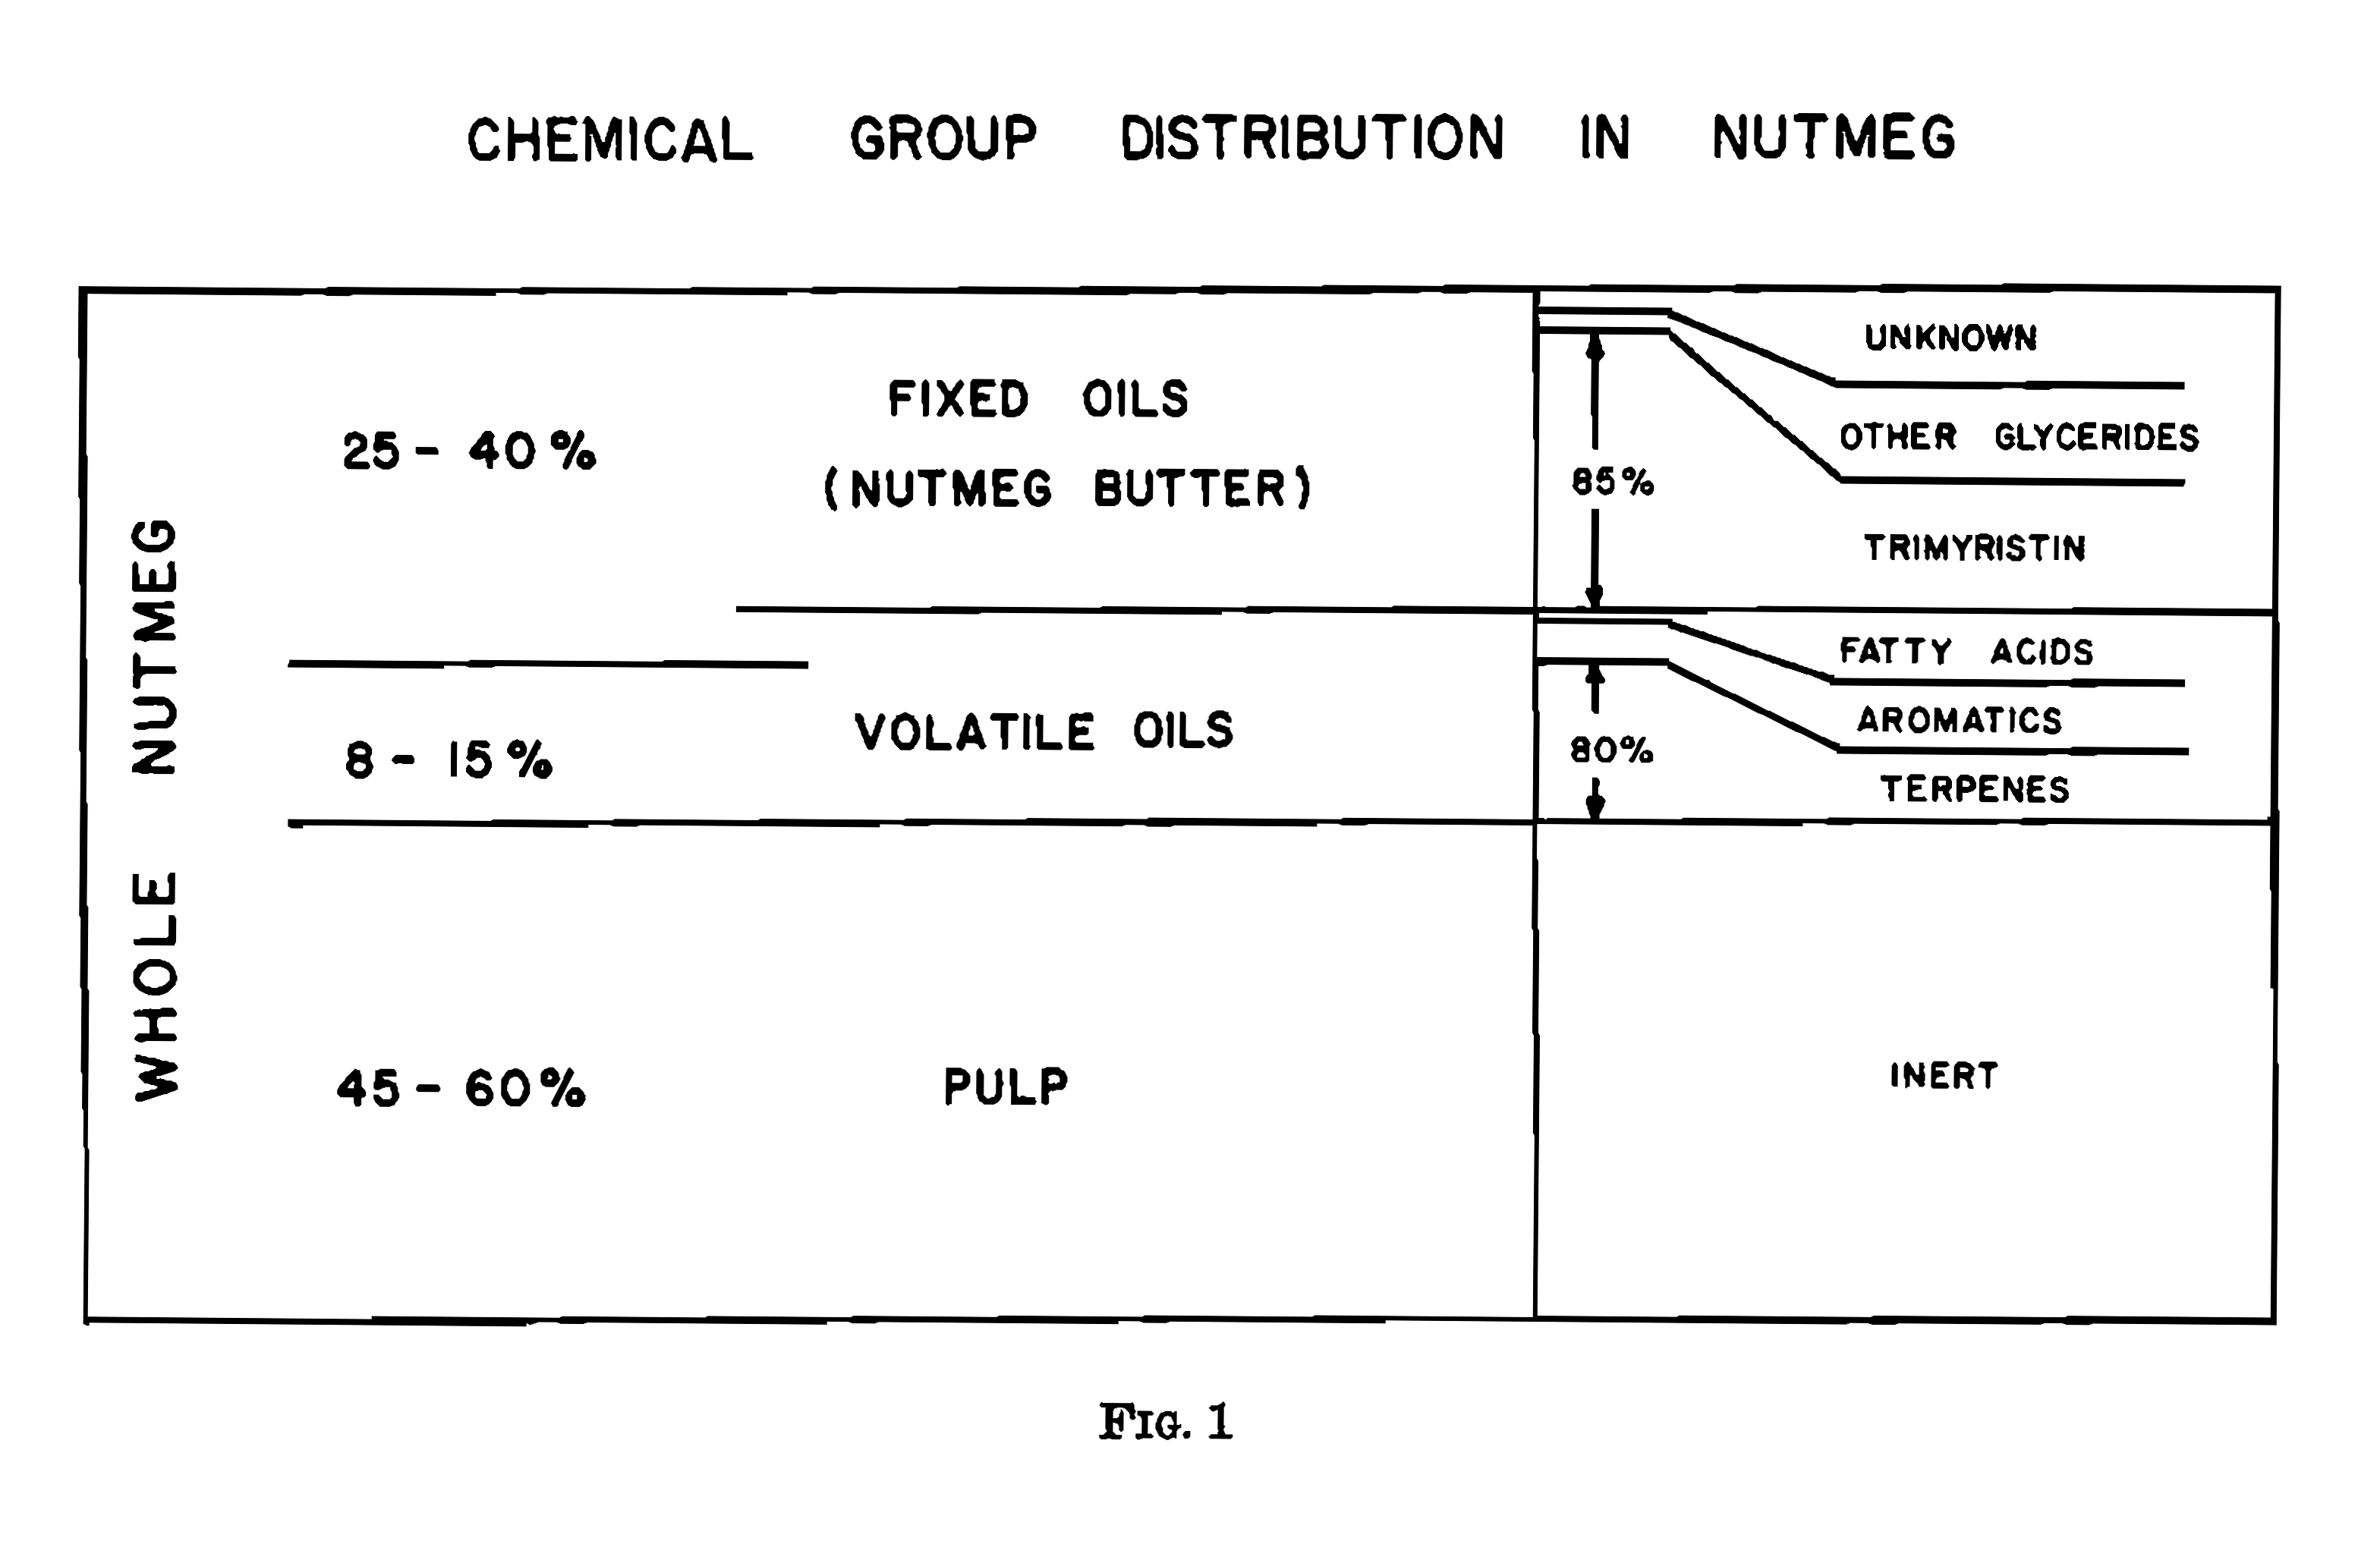
\includegraphics[scale=0.122]{Figure1}


Det som blir kvar efter dessa processer och extraktioner av de flyktiga oljorna utgör till ett ungefär 50\% av den ursprungliga vikten av muskotnöten. Den är förmodligen en cellulosa liknande massa, och den förblir komplett outforskad i form av någon kemisk analys.

Det måste bli fastställt här hur i väntan på kommande diskussion angående farmakologin av muskotnöt att ingen definitiv utvärdering av dessa fraktioner (fetterna och massan) har blivit gjorda. Det är dock, generellt accepterat att det är den flyktiga oljans fraktion som man måste vända sig till för de aktiva beståndsdelarna av muskotnöten, och det är denna ''Olja av Muskotnöt'' som är erkänd av den Amerikanska Farmakopén som en medicin.

Denna flyktiga olja innefattar mellan en åttondel och en tolvtedel av den hela nöten och är saken för denna studie.

\hbox{\hspace{0cm}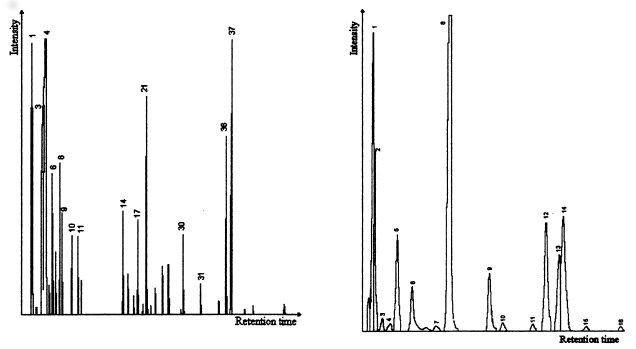
\includegraphics[scale=0.85]{GCgraph}}

\begin{minipage}[t]{2cm}
\flushleft
\textsc{\textbf{Fig. 2}}
\end{minipage}
\hfill
\begin{minipage}[t]{2cm}
\flushright
\textsc{\textbf{Fig. 3}}
\end{minipage}


\begin{table}[!htbp]
\small
\centering
\caption{GC analys av muskotnötens flyktiga olja vid 90 bar - $23\,^{\circ}\mathrm{C}$}
\begin{tabular*}{\textwidth}{l @{\extracolsep{\fill}} @{}cll@{}}
\toprule
Topp nummer & \ Retentions tid (min) & Yta (\%) & Identifikation                                      \\ \midrule
1           & 2.880                & 11.0520   & $\alpha$-pinene                                      \\
3           & 3.898                & 10.1872   & $\beta$-pinene                                       \\
4           & 4.175                & 36.6348   & sabinene                                            \\
6           & 4.763                & 3.1476    & myrcene                                             \\
8           & 5.470                & 3.7710    & limonene                                            \\
9           & 5.655                & 2.2727    & $\beta$-phelandrene                                  \\
10          & 6.545                & 1.8826    & $\gamma$-terpinene                                   \\
11          & 7.097                & 1.6559    & cymene                                              \\
14          & 11.287               & 1.8101    & \textbf{cis*}   \\
17          & 12.658               & 1.7945    & \textbf{trans*} \\
21          & 13.455               & 3.6766    & terpinen-4-ol                                       \\
30          & 16.907               & 1.0075    & safrol                                              \\
36          & 20.907               & 3.2933    & elemicin                                            \\
37          & 21.393               & 6.9835    & myristicin                                          \\ \bottomrule
\end{tabular*}
\note{\textbf{cis*} = 1-methyl-4(1-methylethyl)2-cyclohexen-1-ol (cis)
\\
\textbf{trans*} = 1-methyl-4(1-methylethyl)2-cyclohexen-1-ol (trans)}

\end{table}

En bestämmande analys av denna flyktiga olja har lånats av \cite{spricigo1999extraction}.
Till denna analys användes hela muskotnötter som levererats av Bretzke Alimentos \textit{(Jaragua? do Sul, SC, Brazil)}. De maldes med en kaffekvarn, efter det utfördes
en extraktion av de flyktiga oljorna. Extraktionen utfördes med en ångdestillation enligt metoden beskriven av ``The American Spice Trade Association'' för ett bestämmande av flyktiga oljor
\cite[citerad av Ferreira]{spricigo1999extraction}.
\textbf{Fig. 2} visar en GC analys av den hela flyktiga olje fraktionen erhållen
från proceduren. Tabell 1 visar en identifikation av de större topparna.
Från detta resultat kan det visas hur huvudämnena av den flyktiga oljan är $\alpha$-pinene, $\beta$-pinene, sabinene samt myristicin, den karaktärsgivande aromatiska beståndsdelen av muskotnöt.

\textbf{Fig. 3} utgår, det är en identifikation av de fett syrorna som återfinns i den icke flyktiga olje fraktionen av muskotnöt, tillhörande tabell ingår ej i denna rapport men kan finnas i \cite[s.258]{spricigo1999extraction}

Den mindre gruppen som vi ser i \textbf{Fig. 1}, den aromatiska
eter fraktionen är den mest intressanta av de olika vilket kommer visas senare
och är mer trolig att vara involverad i de psykoaktiva effekterna av
muskotnöt.
De tre huvudkomponenterna av den aromatiska fraktionen är myristicin, elemicin
och safrol vilka står för nästan 9/10 av fraktionen.
I tidigare studier av muskotnöt så har myristicin alltid erkäns som en
huvudbeståndsdel och har därefter trots vara ansvarig för de berusande effekterna.

Uppgiften att tillgodose kemiska strukturer till de olika beståndsdelarna är
en enkel uppgift i jämförelse med uppgiften att tillse ansvar för de
beståndsdelar som bidrar till de berusande och psykotropiska egenskaperna hos muskotnöten.
Kärnan i sig är den enda delen av nöten med ryktet av biologisk aktivitet.
Att de psykoaktiva beståndsdelarna skulle återfinnas hos den flyktiga olje fraktionen av kärnan kan styrkas med att djurstudier visat på att den bibehåller samma verkan som den hela nöten.
Mänskliga experiment med riven muskotnöt tömd på dess flyktiga oljor har
misslyckats med att visa någon form av psykoaktiv respons. \cite{truitt}

Efter en tilldelning av kemiska strukturer till de olika beståndsdelarna
som kan ansvara för effekerna, så måste man undersöka hur var och en, eller
mer troligt tillsammans, kan uppnå rollen till
effekterna vi kan få av den hela nöten.
Vi har två typer av ämnen att betrakta, terpenerna och de aromatiska etrarna.
Det är frestande att direkt utesluta terpenerna fastän de utgör en överväldigande
del av den flyktiga oljan. Terpenernas kolväten är generellt kända som att vara
biologiskt effektiva endast som retmedel.
Terpentin har en sammansättning lik denna terpen fraktion; det har använts
i många huskurer men har visserligen inget rykte som ett berusningsmedel.
Det kan å andra sidan ha någon funktion vid upptagning av olika aromatiska etrar i
magsäcken.


Den aromatiska fraktionen är den som verkar vara den mest troliga källan till de berusande effekterna av muskotnöt. \textbf{Tabell 2} visar strukturerna av varje förening återfunnen i den aromatiska fraktionen. Även visat är mängden i milligram som skulle återfinnas hos 20g av en hel muskotnöt, det antaget vara den dos som krävs
för fullgoda berusande effekter.

\pagebreak

\centered{\caption{\textbf{Tabell 2}}

\hbox{\hspace{0cm}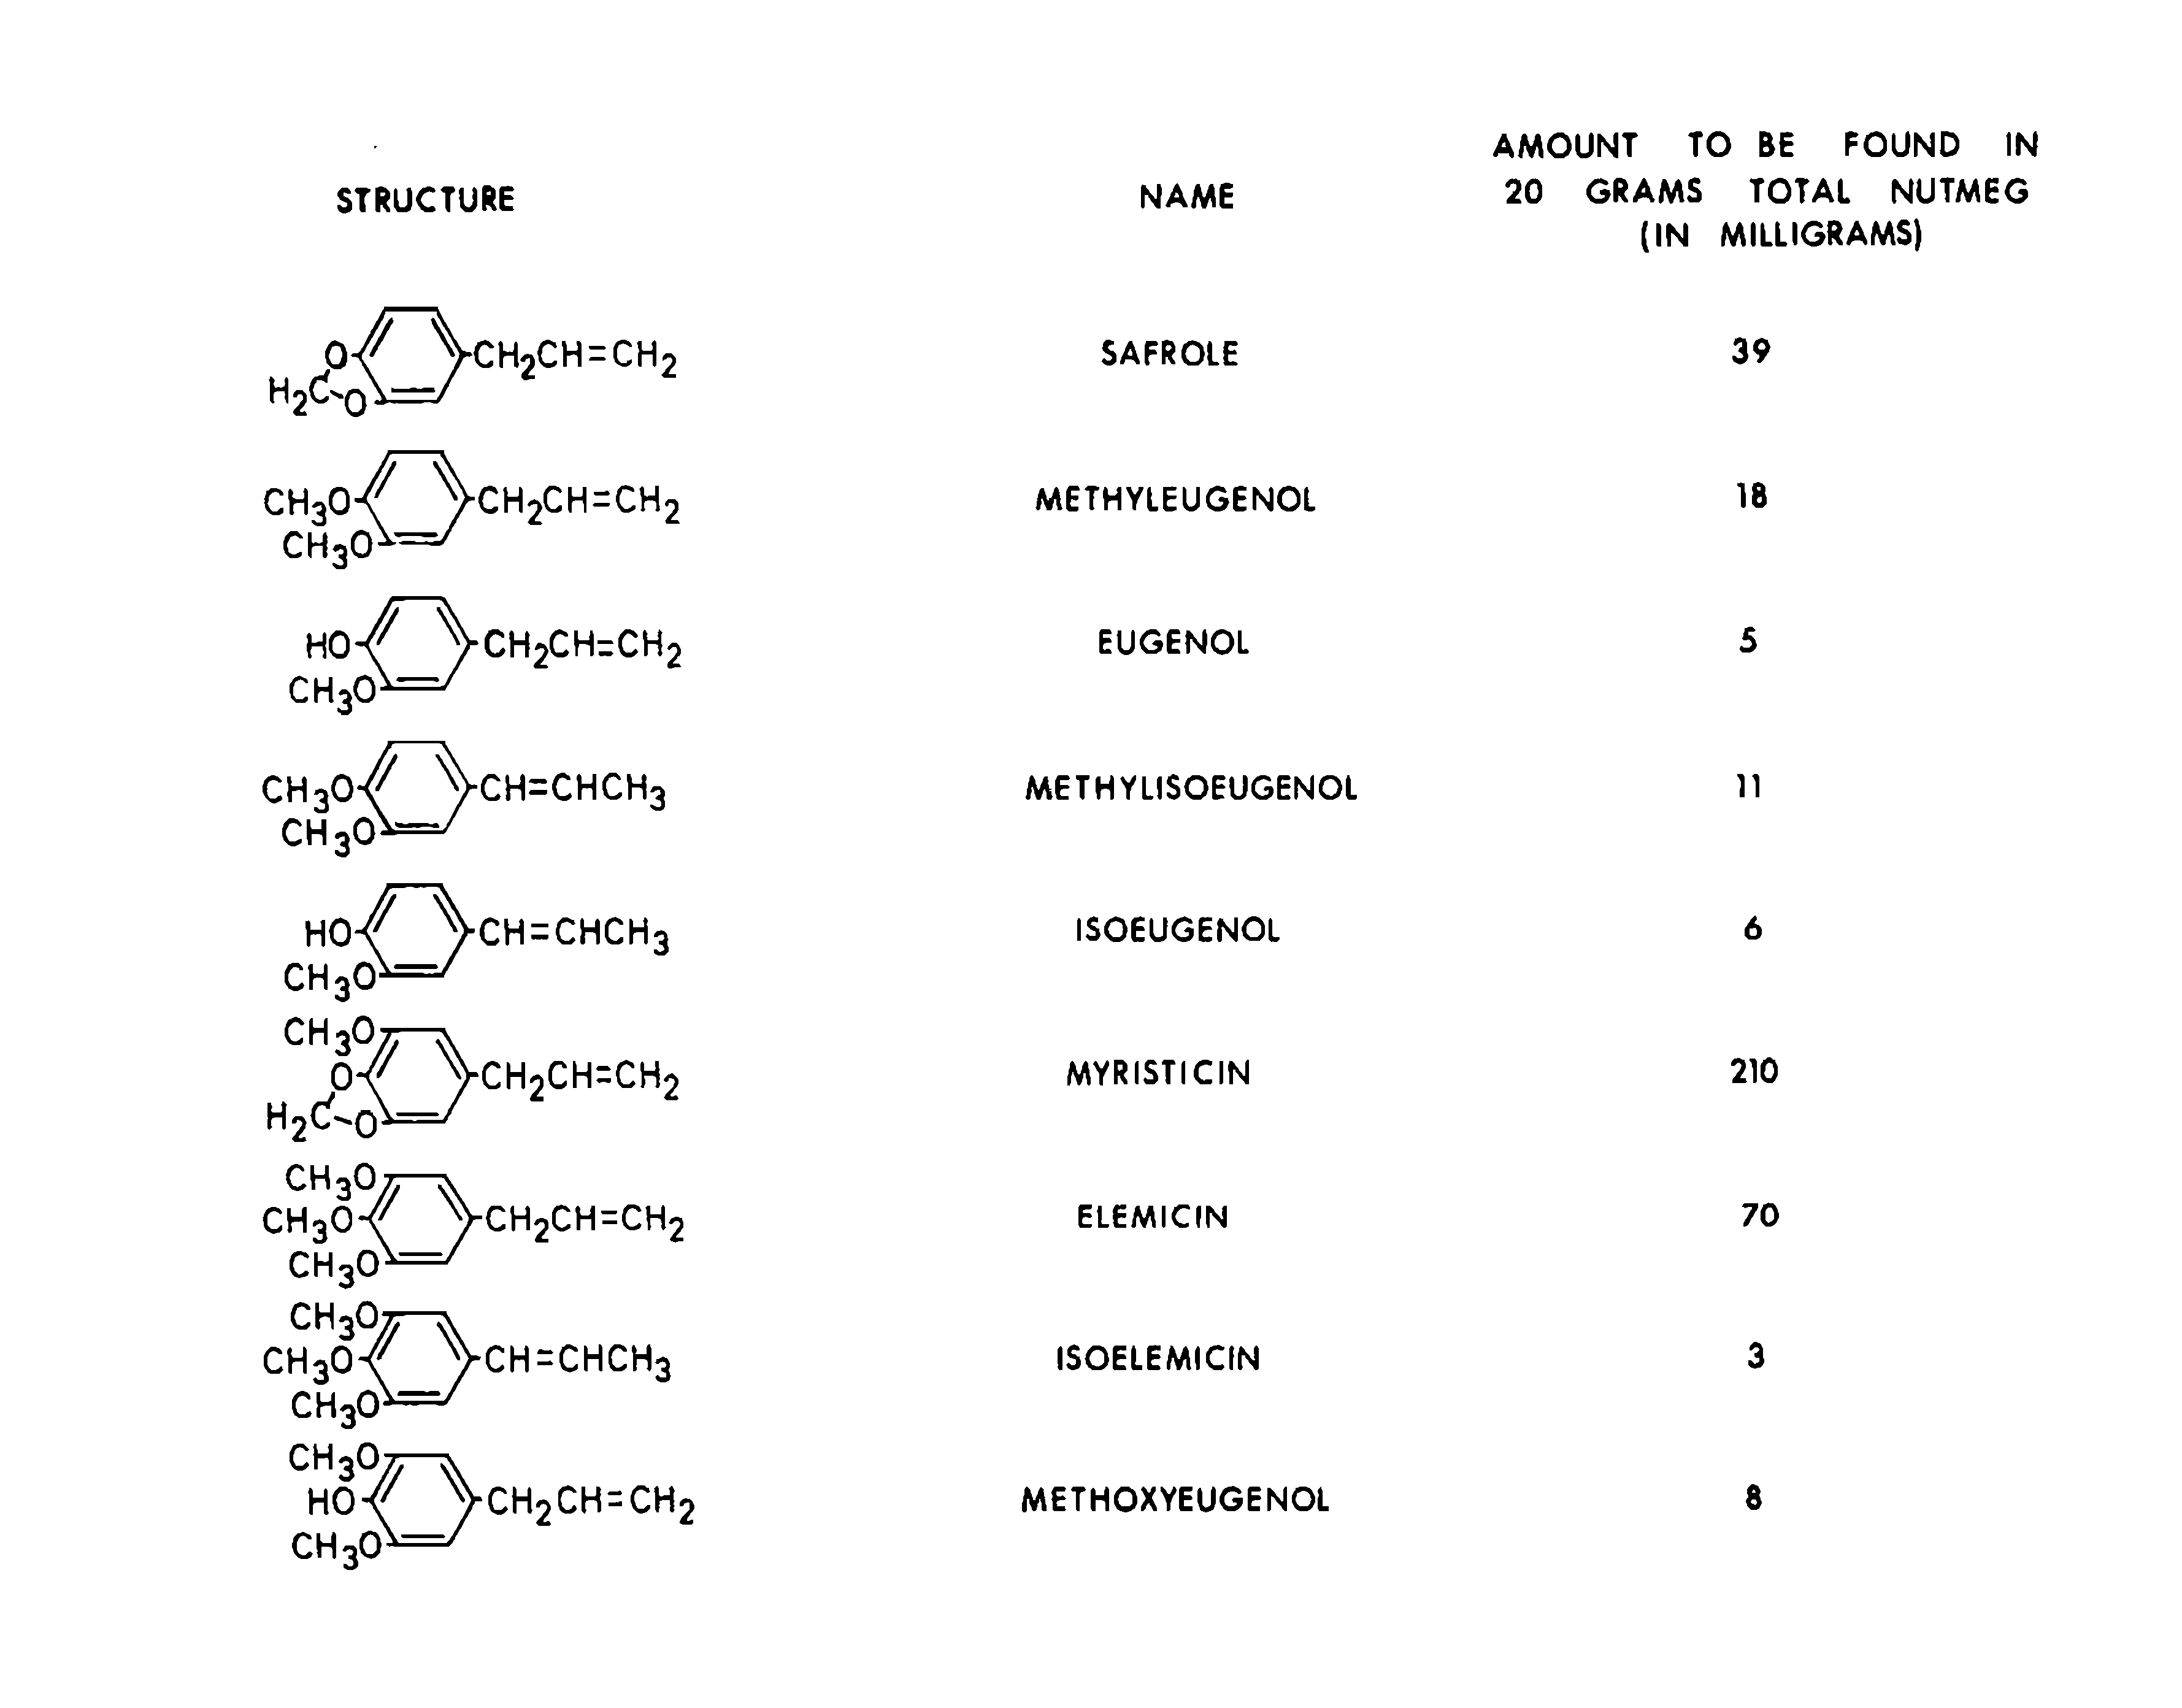
\includegraphics[scale=0.12]{Tabell2}
}

Som fastställt innan så upptar safrol, myristicin, och elemicin 84\% av den
aromatiska fraktionen, och är därefter de huvudsakliga ämnena som vi kommer att överväga.
Dock måste man ha i åtanke om möjligheten att en av de mindre beståndsdelarna
kan ha en ovanligt hög potens och bidra till effekterna.

Av de huvudsakliga beståndsdelarna så är myristicin överlägset den mest förekommande,
av denna anledning så har tester utförts specifikt för psykotropisk effekt av
Truitt, \textit{et al} \cite{truitt}. Doser på 400mg myristicin, nästan det dubbla som förväntas
hos 20 g. av typisk muskotnöt utdelades till frivilliga människor (vad heter detta, svenska) och de observerade symptomen var åtminstonde tydande av psykotropiska effekter hos 6 av 10
försöks personer.

Safrol, även det en beståndsdel av andra naturliga oljor och kryddor, mest känd från oljan från Sassafras trädet vilket safrol utgör 80\% av. Både oljan samt det utvunna Sassafrasteet har använts i en bred utsträckning, måttligt som ett smakämne, och i högre mängder som intern medikament; men varken har något rykte för någon psykotropisk aktivitet vilket muskotnöten har.

Elemicin, det förekommer sällan bland smaksättande oljor och kryddor, ändå så
återfinns det i en relativt stor mängd i muskotnöt. Vidare, vilket kommer tas upp i diskussionen så varierar mängden av elemicin kraftigt och beror på ursprunget av nöten. Elemicin återfinns även bland ett antal obskyra eteriska oljor, inga med någon känd farmakologisk användning. Elemicin är vidare inte separerbar från myristicin vid fraktionell destillation. Myristicinet som använts i all tidigare farmakologi (inklusive de mänskliga experimenten ovan) har ursprungat från destillation av muskotnöts olja och trotts att vara bestående av endast myristicin. Därav så kan vi inte veta om det innehöll elemicin.
Skillnaderna mellan innehållet av elemicin från olika ursprung kan möjligtvis redogöra för den hög diskrepans som återfunnits hos de rapporterade effekterna hos muskotnöt, vilket i sin tur antyder att elemicin kan visserligen vara en aktiv beståndsdel.

Av den aromatiska fraktionen, i mindre beståndsdelar finner vi endast, eugenol och isoeugenol som tidigare använts antingen som smakämnen eller medicin.
De utgör ungefär 80\% av nejlikolja exempelvis, men sökning bland litteraturen angående sådana naturliga produkters rykte som berusning eller missbruksmedel har visat sig vara meningslöst.

Därav finns det flera möjligheter genom vilka de aromatiska beståndsdelarna kan vara involverade som en källa till effekterna.
\begin{enumerate}
	\setlength\itemsep{0em}
\item En av de beståndsdelar som är närvarande i endast väldigt små mängder har en ovanligt hög potens.
\item Elemicin kan vara en större källa av aktivitet än tidigare trott, eller
\item En kombination av två eller fler av aromaterna närvarande är involverad.
\end{enumerate}

%dessa resultat verkar visa en stor diskrepans mellan muskot från olika geografiska källor, gör en komparativ analys, citera shulgin.

%Nu ska jag börja gå in på vad den flyktiga oljan består av och vissa likheter mellan myristicin samt tma osv, norsk källa här.

%Ska infoga figur 2 vilket ska vara en ms/gs graf och förklara den.

%Jag ska komma fram till att muskokot = myristicin/elemicin innan jag börjar med resultatet.

%Vad muskotnöt består av här, grafer osv1

	\subsection{Resultat}

	De tre ämnen som närvarar i störst mängd, myristicin, elemicin och safrol kan vara en tillräcklig förklaring till muskotnötens berusande effekter.

	Det är värt att påpeka att muskotnöt är den enda växtkällan inom vilken dessa tre ämnen förekommer tillsammans i någon avsevärd mängd, vilket som kommer visas senare hur det bidrar med till de olika delarna av den totala effekten.

	Ringsubstitutionen för dessa ämnen från den aromatiska fraktionen är märkv-ärdig då ett flertal av dem, speciellt myristicin, elemecin och safrol, är identiska till ring strukturerna av ämnen med en känd och etablerad psykoaktiv effekt. Den allyliska sido kedjan kan enkelt ändras med hjälp av kemisk modifikation, vilket är visat i Fig. 4, detta skulle kunna omvandla de naturligt förekommande ämnena till de med känd psykoaktiv effekt.

	Det har föreslagits \cite{shulgin1967chemistry}, att tillskottet av ammoniak \textit{in vivo}, vid antingen allyl eller propenyl isomerens alkena ställe skulle erhålla amfetaminer direkt.
	%till det alkena stället på antingen allyl eller propenyl isomeren.
	%\textbf{the in vivo addition of ammonia to the olefinic (alken) site in either the allyl or the propenyl isomer would yield amphetamines directly}.
	Men att tala of amfetaminer som en kemisk klassifikation vore inte helt korrekt, men vi använder ordet för att hänvisa till diverse metoxiderade phenyl-isopropylaminer, även känt som phenetylaminer då de alla bär samma identitetsgivande phenetylamin skelettet.
	``RO'' gruppen i figuren visar på närvarandet av någon form av ester på ringen,	och inkluderar därefter alla de aromatiska estrarna från oljan av muskotnöt men även
	från många andra naturliga oljor.
	Den troliga mekanismen för en sådan \texit{in vivo} modifikation har beskrivits,
	och är trolig till den grad att var och en av reaktionerna utförts \textit{in vitro}.

	Stöd för påståendet om att en modifikation som denna skulle kunna ske \textit{in vivo} har erhållitsav Barfknecht \cite{shulgin1967chemistry}, som funnit bevis på en produktion av amfetaminer i råttor
	efter att ha matat dem med allylbenzene. Detta motsvarar tillskottet av
	ammoniak i Fig. 4 utan ``RO'' ester gruppen.




	\hbox{\hspace{1cm}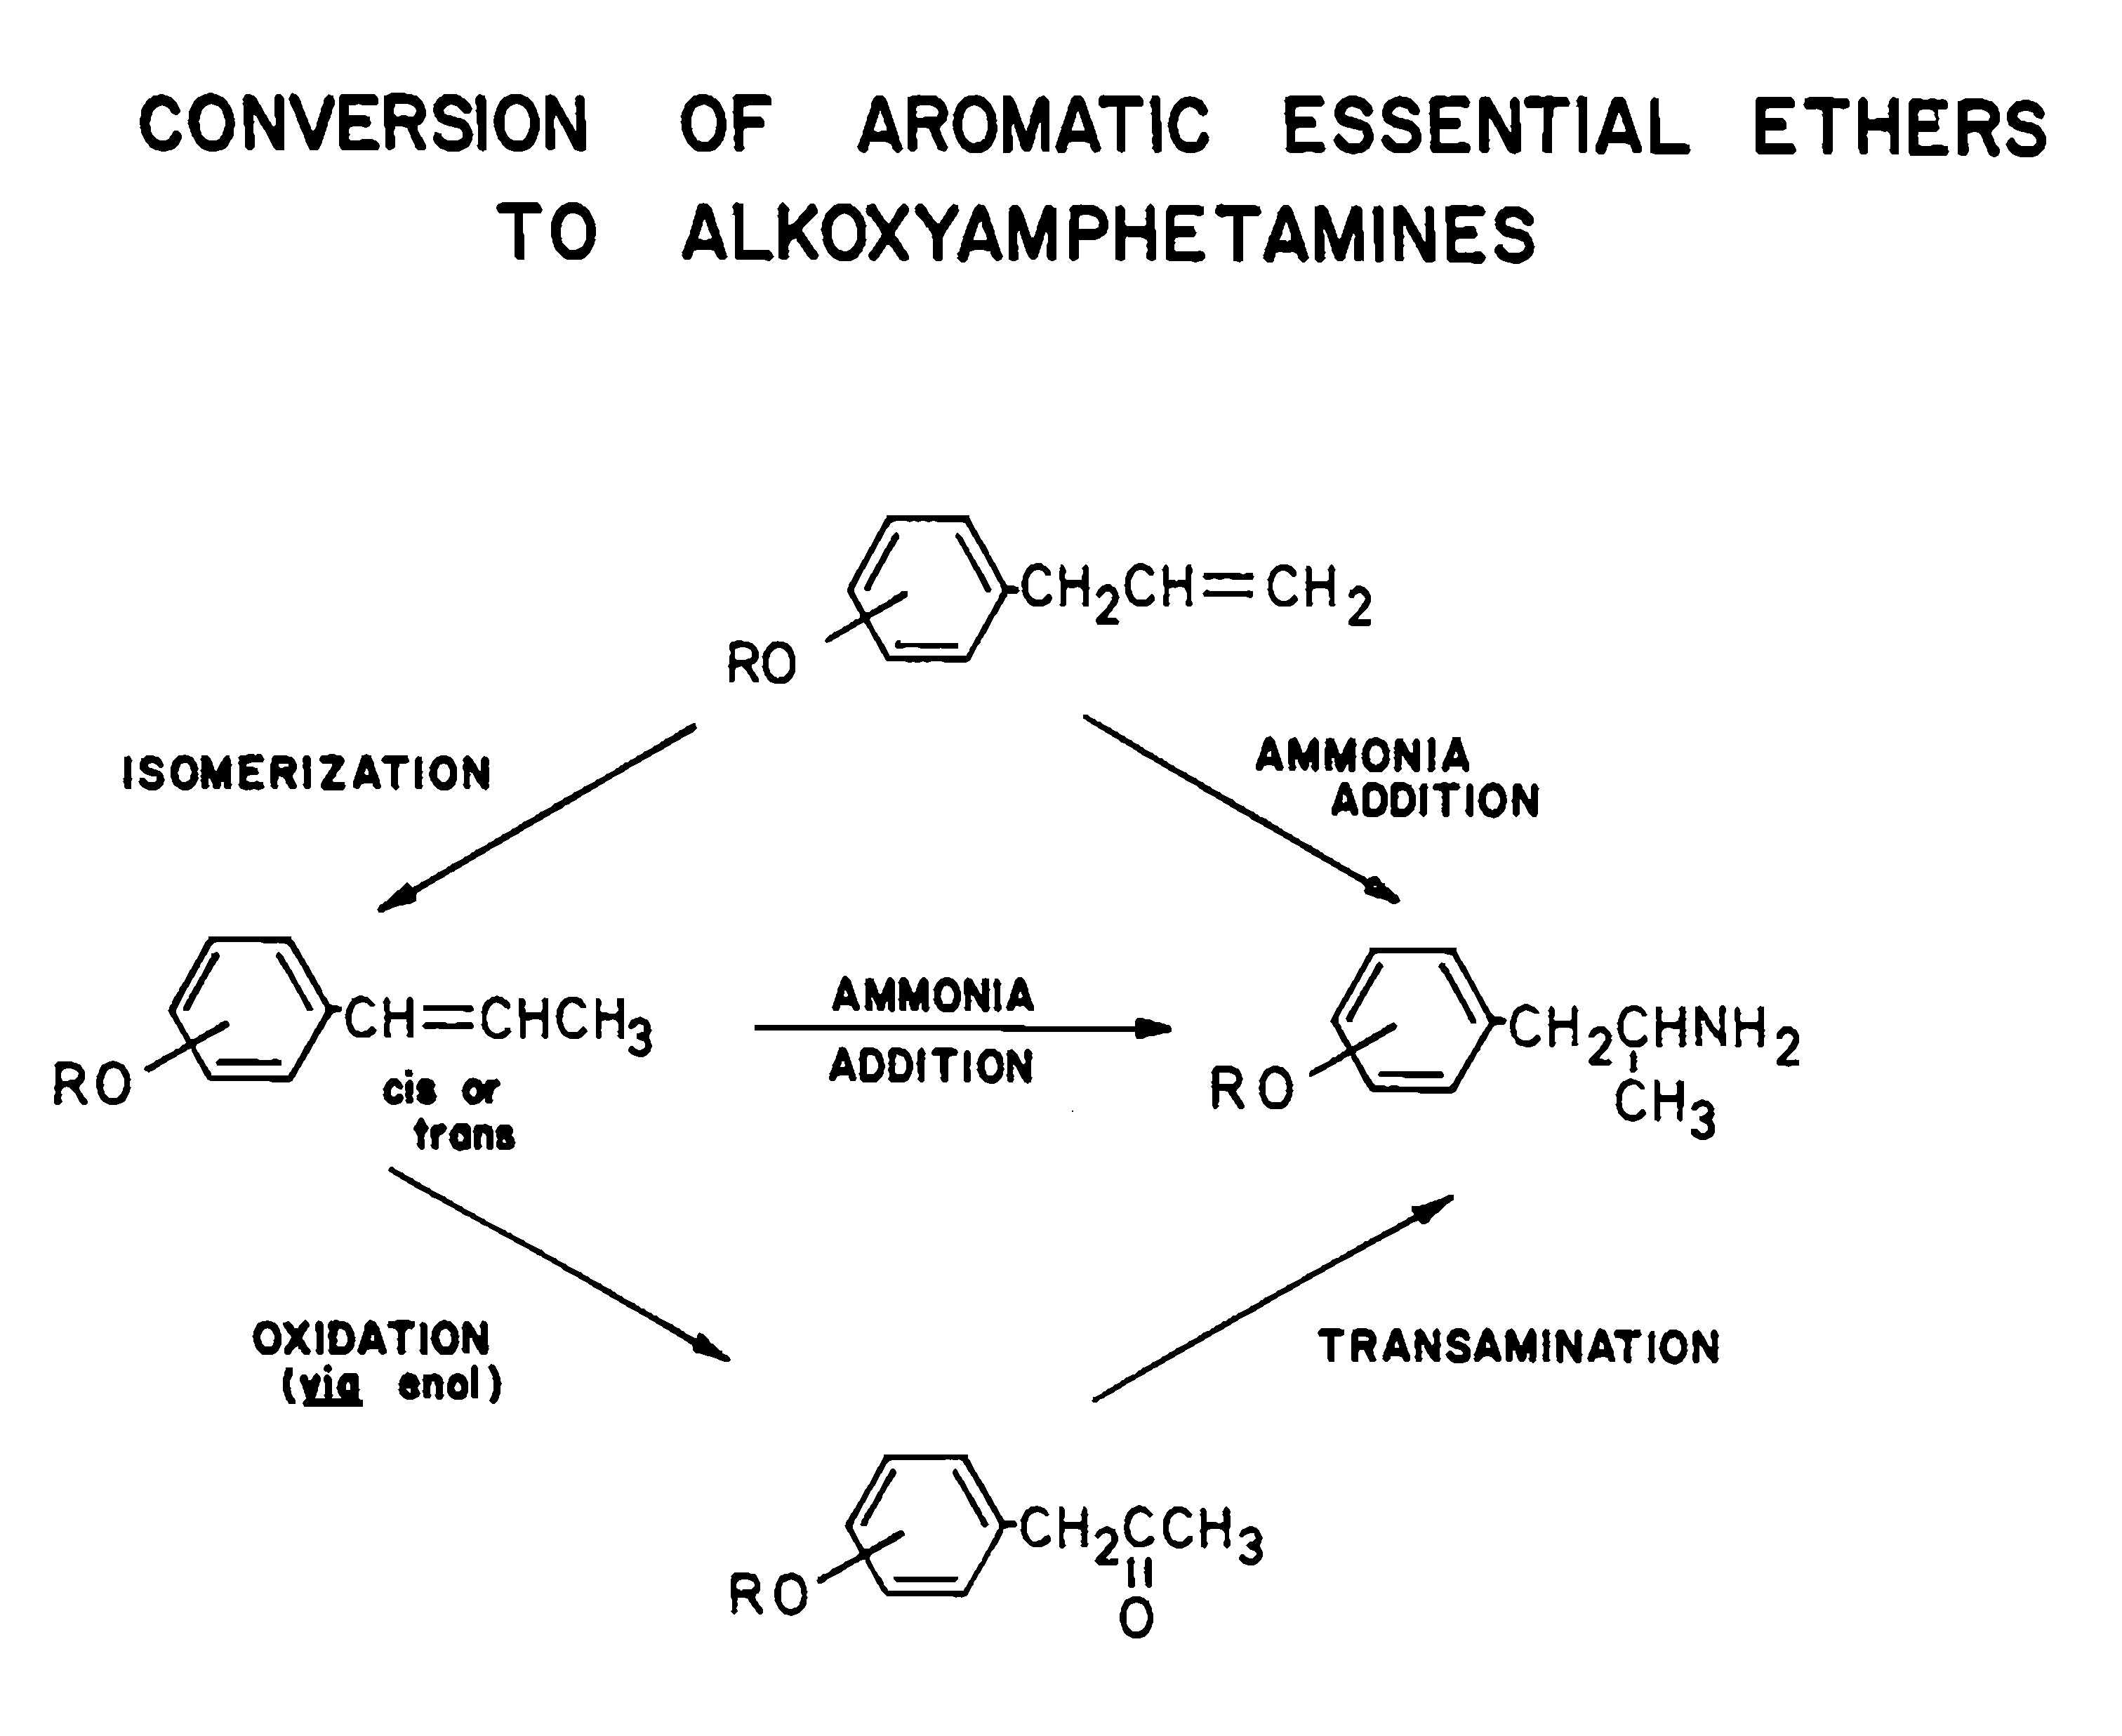
\includegraphics[scale=0.115]{Figure4}
	}
	\begin{center}\textbf{Fig. 4.}\end{center}


	En studie av de möjliga amineringarna \textit{in vivo} av dessa ring substituerade
	ämnen har utförts, de amfetaminer som skulle vara resultaten av en sådan
	aminering har blivit fastställda för de respektive ämnen som återfunnits
	i den aromatiska fraktionen.

	Den bas som korresponderar till safrol, är 3,4-metylendioxiamfetamin, MDA.
	Denna bas var först beskriven farmakologiskt av Gordon Alles \cite{alles1959some} som
	rapporterade visuella effekter vid en dos på 120mg. Ett följande experiment
	\cite{shulgin1967chemistry} på ett mer omfattande antal försökpersoner visade milda, om några
	visuella effekter, men snarare en emotionell verkan, vilket har visat sig
	vara av ett betydande värde för psykoterapi.

	Den bas som skulle vara resultaten av en aminering av myristicin, är
	3-methoxy-4,5-methylenedioxyamphetamine, MMDA.
	Detta är en något okänd substans, med lite om något underlag av mänsklig användning. Men studier har visat likheter till de effekter av tidigare nämnda MDA, men utöver det så har det föreslagits \cite{shulgin1995pihkal}, att det förekommer levande och väl strukturerade hallucinationer vid stängad ögon. Men det var ingen ändring hos förekomsten av hallucinationer vid öppna ögon. En utförlig rapport av den mänskliga farmakologin hos MMDA finns i bilaga 4.
	Men detta visar på att möjligheten att myristicin i de mängder närvarande i muskotnöt skulle bidra till effekterna av muskotnöt inte kan bli avskedade.

	Den bas som skulle resultera från en aminering av elemicin, är
	3,4,5-trimetho-xyamphetamine, TMA. Detta har varit ett känt psykoaktivt medel för en viss tid. \cite{peretz1955new}
	Den har på olika sätt blivit beskriven som kapabel till hallucinogena effekter
	och lett till en synes ovänlig respons. \cite{shulgin1995pihkal}
	Mer utförliga analyser av detta ämne har granskats \cite{shulgin1995pihkal}, och i psykoterapeutiska miljöer så har det fastställts att förväntade effekter innefattar; hallucinationer vid öppna ögon och tillfälliga hörsel hallucinationer.
	Det har även föreslagits att dess karaktärsgivande effekter är just att skapa projekteringar, på pskyologiskt vis hos användaren.
	Detta kan betyda visuell distorsion, inbillningar (förändringar i uppfattningen av sociala situationer), och ibland till synes ovänliga projektioner, vilka dock aldrig orsakat några uppenbara problem.

	\subsection{Diskussion}

Det finns två sätt som vidare studier kan följa; nämligen en mänsklig utvärdering
av varje individuellt ämne från den aromatiska fraktionen av muskotnöts oljan,
helst syntetiskt deriverad för att undvika kontaminering, och för det andra sättet,
en utvärdering av amin baserna deriverade från muskotnötsoljan, alltså
TMA, MMDA och MDA. Dessa skulle kunna förklara de psykologiska effekterna
vi funnit hos muskotnöt. De toxiska effekterna skulle kunna bero på terpen fraktionen
där vi finner cymene vars molekylära uppbygnad liknar camphene som är en känd
carcinogen. En mänsklig utvärdering av en blandning av dessa aminer deriverade från
muskotnöt oljan, i samma proportioner som skulle återfinnas hos muskotnöt skulle
utforska möjligheten av en synergisk förstärkning av aktiviteten hos dessa ämnen.

En följd studie skulle involvera en kemisk utvärdering av ödet efter metaboliseringen
hos de ämnen som återfunnits i den aromatiska fraktionen och dess amin derivator
med en administration hos mänskliga patienter vilket skulle kunna klargöra om dessa
oljor faktiskt metaboliseras till aminer i kroppen, \textit{in vivo}.
Resultatet av en sådan studie skulle förhoppningsvis förklara det
komplexa förhållande som återfinns mellan de ämnen som trotts vara aktiva
hos den hela muskotnöten.


%ta upp att ursprunget gör så att andelen av oljor ändras men bara lite kort
%och skriv kolla för mer i källa ...


\pagebreak

\printbibliography

\pagebreak

\section{Bilagor}
\subsection*{Bilaga 1}

% This is the (pdf)LaTeX source for:
% Erowid Experience Vaults Report Id: 22800
% Copyright (c) 2016 erowid.org
%
% Please contact copyrights@erowid.org for permission to reproduce.
%
%
% This sourcefile was generated by exp_latex.pl v.1.2  using Perl version 5.024001 at Mon Dec 19 12:51:32 2016 GMT on Dec 19 2016

\documentclass[letterpaper,12pt]{article}
\usepackage[letterpaper,left=20mm,right=20mm,bottom=35mm]{geometry}

\setlength{\parindent}{0pt}


\usepackage{ucs}
\usepackage[utf8x]{inputenc}

\usepackage[pdftex]{color,graphicx}
\pdfcompresslevel=9
\DeclareGraphicsExtensions{.png,.jpg,.pdf,.gif}

\usepackage{ifpdf}
\ifpdf
\usepackage{datetime}
\fi

\usepackage{url}

\usepackage{fancyhdr}
\usepackage{hyperref}
\pagestyle{fancy}
\fancyhf{}
\renewcommand{\footrulewidth}{0.4pt}
\fancyhead[L]{\setlength{\unitlength}{1mm}\begin{picture}(4,0) \put(0,-1){\includegraphics*[width=0.5cm]{/www/erowid.org/experiences/images/erologo_1cm_600dpi_greyscale}} \end{picture} \footnotesize\sffamily Erowid Experience ID: 22800}
\fancyhead[C]{\footnotesize\sffamily Keeping it Real ...  My Nuts!}
\fancyhead[R]{\footnotesize\sffamily by Transambulance}

\fancyfoot[L]{\footnotesize\sffamily Exp Year: 2003\hspace{0.2cm} Added to Database: Oct 4, 2006\\ Gender of reportee: male\\ \vspace{0.1cm} \scriptsize\sffamily Generated by exp\_latex.pl v.1.2  using perl \& pdf\LaTeX \\ on Mon Dec 19 12:51:32 2016 GMT.}
\fancyfoot[C]{\\ \vspace{0.5cm} \\ \thepage}
\fancyfoot[R]{\footnotesize\sffamily \url{https://www.erowid.org/experiences/exp.php?ID=22800} \\ \vspace{0.1cm} \copyright\,2016 by \href{https://www.erowid.org}{erowid.org}}

\fancypagestyle{plain}{
\fancyhf{}
\renewcommand{\headrulewidth}{0pt}
\fancyfoot[L]{\footnotesize\sffamily Exp Year: 2003\hspace{0.2cm} Added to Database: Oct 4, 2006\\ Gender of reportee: male\\ \vspace{0.1cm} \scriptsize\sffamily Generated by exp\_latex.pl v.1.2  using perl \& pdf\LaTeX \\ on Mon Dec 19 12:51:32 2016 GMT.}
\fancyfoot[R]{\footnotesize\sffamily \url{https://www.erowid.org/experiences/exp.php?ID=22800} \\ \vspace{0.1cm} \copyright\,2016 by \href{https://www.erowid.org}{erowid.org}}}

\makeatletter
\renewcommand{\fnum@figure}[1]{}
\makeatother


\begin{document}

\ifpdf
\pdfinfo{
/Title (Erowid Experience Vaults Report Id: 22800 Experience Year: 2003)
/Subject (Keeping it Real ...  My Nuts!)
/Author (Transambulance)
/Creator (pdfLaTeX)
/Producer (erowid.org)
/CreationDate (D:\pdfdate)
/Keywords ()
}
\fi

\section*{\begin{picture}(20,0) \put(-5,-10){\includegraphics*[width=1cm]{/www/erowid.org/experiences/images/erologo_1cm_600dpi_greyscale}} \end{picture} Erowid Experience Vaults Report Id: 22800}

\subsection*{Keeping it Real ...  My Nuts!}
\vspace{-0.2cm}
by \emph{Transambulance}
\vspace{0.5cm}
\thispagestyle{plain}

\setlength{\parskip}{1ex}
\begin{tabular}[h]{|c|c|c|c|c|}
\hline
Dose:  T+ 0:00 & 2 seeds & oral & Nutmeg & ground / crushed\\
\hline
\end{tabular}

\vspace{1mm}

\begin{tabular}[h]{|c|c|}
\hline
Body weight: & 160 lbs\\
\hline
\end{tabular}

\vspace{2mm}
I can attest to the effects of nutmeg, and I will certainly repeat the experience.  Before I started this little adventure, here are the tips I was able to gather from online research.



1.  Don't use powder, use whole, fresh, organic nutmeg

2.  Don't underestimate its potency; most people take way too much

3.  Expect 3-4 hours to pass between ingestion and effects

4.  Clear your calander for at least 36 hours after ingestion

5.  Figure out a way to get it down; the taste is awful

6.  Watch out for dehydration and a killer hangover



Here's what I did:



Ingestion



I crushed two fresh nuts, purchased from a local organic co-op, in a steel pot with a hammer, wrapped each of the three resulting teaspoons of mash in a melted-mozzerella-cheese-slug, which I then swallowed whole.  The taste of nutmeg is unpleasent, but the cheese-slugs acted like a large pill-casings.  Pure lemon juice worked to wash out the worst of the flavor, but I had nutmeg-flavored burps for a while afterwards.



The Experience



1.  Euphoria



The first giggles set in three hours after ingestion.  I felt drowsy, and when I allowed myself to relax, everything seemed funny.  Early on, the experience was very similar to mellow marijuana or marijuana and alchohol at the same time.  Giggles and good feelings were easy to control, but enjoyable when left uncontrolled.  I watched the Sunday night edition of Adult Swim, and was much less critical of it than I usually am (marijuana has this same effect on me).



2.  Hallucinations



I had lots of `good ideas' (ideas that are fun to think about and mentally explore) on Nutmeg.  I get `good ideas' from marijuana, but my thinking was different on Nutmeg.  As the experience continued, I found myself experiencing mild hallucinations and extreme sexual arousal.  I attribute my arousal to the nature of my hallucinations, but others have reported sexual arousal from nutmeg as well.  Hallucinations were quite easy to control once I accepted that I was, in fact, hallucinating, so perhaps they were of an erotic nature because I was aroused by the nutmeg to begin with.



3.  Sedation



Nutmeg made me sleepy and uncoordinated.  This effect seemed tied to the euphoria, but wasn't as easy to control.  I could not concentrate or perform complex motor functions, and `focusing' just made it worse.  Short-term memory was impaired, and it was difficult to get anything done.  This is probably why nutmeg is not a party drug.  This effect lasted the full 36 hours.  You may want to keep at least this much time open if you want a good experience.



Side-Effects and Remedies



1.  Bad Taste



To avoid the taste, I melted fresh mozzerella on a plate, poured the nutmeg mash into three teaspoon-sized lines, and then melted more more fresh mozzerella over the top of each line.  After pinching the cheese fully shut around the spice, I scraped the three `slugs' off the plate and swallowed them whole, one at a time.  The taste was still unpleasent, but not nearly as unpleasent as the raw spice.



2.  Dehydration



The worst side-effect in my experience was cotton-mouth.  I was pissing like a racehorse and dehydrating rapidly once the effects set in, and the cotton-mouth was a good thirst-indicator.  I stopped drinking water at some point, but I kept urinating; more water came out of me than I was putting in, so I forced myself to drink more.  I'd suggest having a good amount of fresh, high-quality water to drink on hand, and drinking enough so your piss stays clear.



3.  Gastro-intestinal disturbance



As I said before, I had nutmeg-flavored burps.  I also had stomach pain and bad gas around eight hours after ingestion, but a slice of fresh ginger under my tongue had me feeling better almost instantly.  I also had lots of stomach-gurgling throughout the experience and an almost non-existant appetite the next day.



4.  The Crash



I had severe fatigue on the following day, similar to a hangover after a night of good fun.  Food (despite my loss of appetite), bed-rest, a hit of marijuana, a bottle of beer at dinner-time, and vegetating in front of cartoons helped me through this.  I think it was worth it, but I had been expecting it to be much worse, based on what I've read.



Suggestions



1. Respect the Nutmeg



Nutmeg isn't as cool as other drugs precisely because it is legal.  It isn't any weaker.  From a psychoactive-benefit and physical-cost standpoint, I found nutmeg to be comparable to a two-mushroom, two-joint, twelve-beer bender.  From a financial-cost and legal-risk standpoint, the nutmeg cost me less than 30 cents and bore zero legal risk.  Everyone weights such things differently, so do your own math.  I think it was more than worthwhile, but I won't go as far as to say that nutmeg is a substitute for any other chemical experience.  Nutmeg is its own experience; respect all parts of that experience and you shouldn't be disappointed.



2. Expect to make a weekend of it



Eating nutmeg is not something to be taken lightly.  I was not expecting nearly as much mental fun as I experienced, but I had prepared myself for the hangover, and I'm glad for that.  I wouldn't have been able to work or attend school the next day, but I could've gone out partying the next night without too many problems.  I feel like nutmeg would be a lot of fun to take on a camping trip with friends, but I wouldn't want to do anything other than chill out the day after the experience.



3. Drink pure water, and lots of it



I was drinking apple juice and tap water.  I normally don't mind my tap water, but the chemical taste bothered me when I had to keep drinking it constantly.  The juice was a big mistake; I wound up with a stomach-ache from guzzling it all too quickly.  I went through a lot of water, and visited the restroom about once every half-hour.  Next time, I will make an herbal tea of fresh ginger with lemon and honey to go with the nutmeg.  The effectiveness of spicy-fresh ginger to relieve nausea surprised me almost as much as the nutmeg did.



Final Analysis



Nutmeg is a powerful psychoactive drug.  From what I've read, most of the negative online reports regarding nutmeg seem to come from people who took too much, expected too much, or who complain too much.  I, for one, hate tracking down illegal drugs and overpaying dealers for them, so I'll be doing this again as soon as I feel up to it.

\end{document}
\pagebreak
\subsection*{Bilaga 2}

% This is the (pdf)LaTeX source for:
% Erowid Experience Vaults Report Id: 15836
% Copyright (c) 2017 erowid.org
%
% Please contact copyrights@erowid.org for permission to reproduce.
%
%
% This sourcefile was generated by exp_latex.pl v.1.2  using Perl version 5.024001 at Tue Jan  3 20:54:46 2017 GMT on Jan 03 2017

\documentclass[letterpaper,12pt]{article}
\usepackage[letterpaper,left=20mm,right=20mm,bottom=35mm]{geometry}

\setlength{\parindent}{0pt}

\usepackage{ucs}
\usepackage[utf8x]{inputenc}

\usepackage[pdftex]{color,graphicx}
\pdfcompresslevel=9
\DeclareGraphicsExtensions{.png,.jpg,.pdf,.gif}

\usepackage{ifpdf}
\ifpdf
\usepackage{datetime}
\fi

\usepackage{url}

\usepackage{fancyhdr}
\usepackage{hyperref}
\pagestyle{fancy}
\fancyhf{}
\renewcommand{\footrulewidth}{0.4pt}
\fancyhead[L]{\setlength{\unitlength}{1mm}\begin{picture}(4,0) \put(0,-1){\includegraphics*[width=0.5cm]{/www/erowid.org/experiences/images/erologo_1cm_600dpi_greyscale}} \end{picture} \footnotesize\sffamily Erowid Experience ID: 15836}
\fancyhead[C]{\footnotesize\sffamily A Portal to Dreams}
\fancyhead[R]{\footnotesize\sffamily by Stahrgazer}

\fancyfoot[L]{\footnotesize\sffamily Exp Year: 2002\hspace{0.2cm} Added to Database: May 4, 2005\\ Gender of reportee: female\\ \vspace{0.1cm} \scriptsize\sffamily Generated by exp\_latex.pl v.1.2  using perl \& pdf\LaTeX \\ on Tue Jan  3 20:54:46 2017 GMT.}
\fancyfoot[C]{\\ \vspace{0.5cm} \\ \thepage}
\fancyfoot[R]{\footnotesize\sffamily \url{https://www.erowid.org/experiences/exp.php?ID=15836} \\ \vspace{0.1cm} \copyright\,2017 by \href{https://www.erowid.org}{erowid.org}}

\fancypagestyle{plain}{
\fancyhf{}
\renewcommand{\headrulewidth}{0pt}
\fancyfoot[L]{\footnotesize\sffamily Exp Year: 2002\hspace{0.2cm} Added to Database: May 4, 2005\\ Gender of reportee: female\\ \vspace{0.1cm} \scriptsize\sffamily Generated by exp\_latex.pl v.1.2  using perl \& pdf\LaTeX \\ on Tue Jan  3 20:54:46 2017 GMT.}
\fancyfoot[R]{\footnotesize\sffamily \url{https://www.erowid.org/experiences/exp.php?ID=15836} \\ \vspace{0.1cm} \copyright\,2017 by \href{https://www.erowid.org}{erowid.org}}}

\makeatletter
\renewcommand{\fnum@figure}[1]{}
\makeatother


\begin{document}

\ifpdf
\pdfinfo{
/Title (Erowid Experience Vaults Report Id: 15836 Experience Year: 2002)
/Subject (A Portal to Dreams)
/Author (Stahrgazer)
/Creator (pdfLaTeX)
/Producer (erowid.org)
/CreationDate (D:\pdfdate)
/Keywords ()
}
\fi

\section*{\begin{picture}(20,0) \put(-5,-10){\includegraphics*[width=1cm]{/www/erowid.org/experiences/images/erologo_1cm_600dpi_greyscale}} \end{picture} Erowid Experience Vaults Report Id: 15836}

\subsection*{A Portal to Dreams}
\vspace{-0.2cm}
by \emph{Stahrgazer}
\vspace{0.5cm}
\thispagestyle{plain}

\setlength{\parskip}{1ex}
\begin{tabular}[h]{|c|c|c|c|c|}
\hline
Dose:  & 2.5 Tbsp & oral & Nutmeg & ground / crushed\\
\hline
\end{tabular}

\vspace{1mm}

\begin{tabular}[h]{|c|c|}
\hline
Body weight: & 160 lbs\\
\hline
\end{tabular}

\vspace{2mm}
My boyfriend and I decided to try nutmeg after reading about its interesting effects.  We paid \$1.19 for 1 small package of whole nutmeg purchased at our local health food market, which when grated equaled about 5 tablespoons.  We then we filled 80 size `O' gel caps with the now powdered nutmeg using my ``cap-M-quik'' capsule filler.   At approximately 4:30 in the afternoon on the 3rd of July, we proceeded to swallow 40 capsules a piece of freshly ground nutmeg, which was about 2 1/2 tablespoons each.

It was an unusually warm 3rd of July for this Coos Bay, OR, so we decided to go play at the Bastendorf Beach awhile before going to the fireworks eve show later on at the Mill Casino.  We splashed in the cold ocean and ran up and down the beach while the kids climbed rocks and built sand cities. It was getting close to dinnertime so we decided to head home\ldots the time was about 6:15 and as my boyfriend started the car he looked at me and said ``I'm starting to feel altered.''   All I could do was grin, as I was starting to feel very calm and ``floaty'', kind of like weed yet\ldots not quite.



While preparing dinner, eating, (which by the way didn't seem to diminish the effects), and getting the kids ready to go out the door, I noticed an increasing peaceful-tingly kind of feeling, nothing too dramatic but definitely ``altered'' and definitely becoming more pronounced. I noticed my heart beat more and my eyes were getting red and sensitive. My talkative move-around-type of boyfriend was kicking back all smiley in the recliner.



What I liked about this trip was the gentle way it came on.  By the time we made it to the fireworks, through the traffic and the crowds at the boardwalk by the casino, we were pleasantly frying.  As we were weaving our way through the crowds, holding tightly to the kids' hands and each other, all we could do was grin at everybody. The fireworks show started right at 10:00, and it seemed the nutmeg kicked in at exactly the right time, because when combined with the fireworks I personally was taken to another world.  Of course fireworks are beautiful anyway, but combined with such a pleasant tingly feeling and beautifully altered perception, they became a portal to dreams. I can't speak for what my boyfriend was feeling at that time, but he just stared and stared at the fireworks, in awe, as he held onto my hand\ldots and he kept that grin on his face.



After coming home and tucking the kids in, we stayed up for several more hours in our bedroom\ldots I am not sure exactly how late because we lost track of time all together. The conversation and laughter flowed well into the night I assure you. We listened to Pink Floyd.  We had taken no other consciousness altering substances that day or that evening.  I don't know if this next comment is appropriate for this forum or not, but since we are talking about the effects of nutmeg I have to mention how good it felt to make love under its effects.  Not only was the sensitivity in our minds heightened, but also the sensitivity of all of our senses.  Nutmeg also produced such a general open, good, loving feeling\ldots like that of a gentle fry\ldots well you can see how the combination would lead to really good sex.  :-)



The next day was actually the 4th of July, and let me tell you when we woke up we realized that the trip wasn't over.  First of all, waking up in itself was a Herculean effort\ldots plus my eyes were all heavy from being so red the night before, they were now very swollen and puffy.  However other than having NO energy at all, the feeling was still pleasant.  We had planned to spend the entire day at the beach into the evening, but it took us 4 hours to pack the car\ldots so we left about 4 that afternoon.  So basically 24 hours after taking the stuff, we were STILL high from it!  The beach was cool.  (We were still so peaceful and happy that I imagine just about anything would have been cool.) We smoked a little weed and shared a bottle of wine with a friend, but still the nutmeg was `the main buzz' so to speak.  We cooked steaks over an open fire, played in the ocean and sand, and lit our fireworks at dusk.  We left the beach around 11 that night then came home and fell asleep nearly as soon as our heads hit the pillow.



Well that was last night, and here on the morning of the 3rd day, we are still coming down.  I can't say I feel unpleasant, but I can tell you I have laid around all day.  I did manage to clean our birds' cages and water the yard, that is it. My poor boyfriend had to go to work today, he just came in for his lunch break and I asked him about his day, he said he didn't know, as he seemed to be sleeping through it. :-)



If one decides to try nutmeg, one might plan on having at least 3 days blocked out of the schedule for it. I needed at least the next day to be free from having to do anything that required hard work or following a schedule. It puts me on a ``void-of-course' feeling. I feel it is on the same level as mushrooms\ldots harmless if used correctly, but not something I'd want to do on a constant basis. Although most people I've read about took 3 tablespoons, I was happy with 2 1/2. It is definitely a consciousness altering high; one I feel would be conducive to meditation or prayer. I wouldn't want to do it alone simply because it gave me a feeling of wanting to share, not isolate.  And I really recommend capsuling it\ldots how people have ever managed just to swallow it is beyond me!

\end{document}
\pagebreak
\subsection*{Bilaga 3}

% This is the (pdf)LaTeX source for:
% Erowid Experience Vaults Report Id: 107415
% Copyright (c) 2017 erowid.org
%
% Please contact copyrights@erowid.org for permission to reproduce.
%
%
% This sourcefile was generated by exp_latex.pl v.1.2  using Perl version 5.024001 at Mon Jan  2 14:23:35 2017 GMT on Jan 02 2017

\documentclass[letterpaper,12pt]{article}
\usepackage[letterpaper,left=20mm,right=20mm,bottom=35mm]{geometry}

\setlength{\parindent}{0pt}

\usepackage{ucs}
\usepackage[utf8x]{inputenc}

\usepackage[pdftex]{color,graphicx}
\pdfcompresslevel=9
\DeclareGraphicsExtensions{.png,.jpg,.pdf,.gif}

\usepackage{ifpdf}
\ifpdf
\usepackage{datetime}
\fi

\usepackage{url}

\usepackage{fancyhdr}
\usepackage{hyperref}
\pagestyle{fancy}
\fancyhf{}
\renewcommand{\footrulewidth}{0.4pt}
\fancyhead[L]{\setlength{\unitlength}{1mm}\begin{picture}(4,0) \put(0,-1){\includegraphics*[width=0.5cm]{/www/erowid.org/experiences/images/erologo_1cm_600dpi_greyscale}} \end{picture} \footnotesize\sffamily Erowid Experience ID: 107415}
\fancyhead[C]{\footnotesize\sffamily  Trance-Dream Scenery and Going Through Hell}
\fancyhead[R]{\footnotesize\sffamily by Jack McQuade}

\fancyfoot[L]{\footnotesize\sffamily Exp Year: 1959\hspace{0.2cm} Added to Database: Jun 10, 2016\\ Gender of reportee: male\\ \vspace{0.1cm} \scriptsize\sffamily Generated by exp\_latex.pl v.1.2  using perl \& pdf\LaTeX \\ on Mon Jan  2 14:23:35 2017 GMT.}
\fancyfoot[C]{\\ \vspace{0.5cm} \\ \thepage}
\fancyfoot[R]{\footnotesize\sffamily \url{https://www.erowid.org/experiences/exp.php?ID=107415} \\ \vspace{0.1cm} \copyright\,2017 by \href{https://www.erowid.org}{erowid.org}}

\fancypagestyle{plain}{
\fancyhf{}
\renewcommand{\headrulewidth}{0pt}
\fancyfoot[L]{\footnotesize\sffamily Exp Year: 1959\hspace{0.2cm} Added to Database: Jun 10, 2016\\ Gender of reportee: male\\ \vspace{0.1cm} \scriptsize\sffamily Generated by exp\_latex.pl v.1.2  using perl \& pdf\LaTeX \\ on Mon Jan  2 14:23:35 2017 GMT.}
\fancyfoot[R]{\footnotesize\sffamily \url{https://www.erowid.org/experiences/exp.php?ID=107415} \\ \vspace{0.1cm} \copyright\,2017 by \href{https://www.erowid.org}{erowid.org}}}

\makeatletter
\renewcommand{\fnum@figure}[1]{}
\makeatother


\begin{document}

\ifpdf
\pdfinfo{
/Title (Erowid Experience Vaults Report Id: 107415 Experience Year: 1959)
/Subject ( Trance-Dream Scenery and Going Through Hell)
/Author (Jack McQuade)
/Creator (pdfLaTeX)
/Producer (erowid.org)
/CreationDate (D:\pdfdate)
/Keywords ()
}
\fi

\section*{\begin{picture}(20,0) \put(-5,-10){\includegraphics*[width=1cm]{/www/erowid.org/experiences/images/erologo_1cm_600dpi_greyscale}} \end{picture} Erowid Experience Vaults Report Id: 107415}

\subsection*{ Trance-Dream Scenery and Going Through Hell}
\vspace{-0.2cm}
by \emph{Jack McQuade}
\vspace{0.5cm}
\thispagestyle{plain}

\setlength{\parskip}{1ex}
\begin{tabular}[h]{|c|c|c|c|c|}
\hline
Dose:  T+ 0:00 & 2 tsp & oral & Nutmeg & ground / crushed\\
\hline
\end{tabular}

\vspace{1mm}

\begin{tabular}[h]{|c|c|}
\hline
Body weight: & 125 lbs\\
\hline
\end{tabular}

\vspace{2mm}
Mace Trip

I was a junior in college, when a ``cool guy'' came to visit one weekend. He inquired if we had any dope, but we didn't. So he suggested we go get some at the grocery store. Three of us went there with him and came back with 3 containers of ground mace. He explained that this substance is prepared from the arillus that grows around the outside of a nutmeg seed, and assured us it is a powerful psychedelic. Back in our dorm each of us took about two heaping teaspoons of the stuff with perhaps 6 oz of water. Nothing happened to me at first, but after half an hour I started to feel a bit dizzy. It occurred to me it would be nice to have some music to accompany the anticipated ``trip''.  I didn't have any music equipment, so I locked myself in the room of another friend who had a record player and was away for the weekend, \& started up some of his Spanish-American music.

Lying on his bed, my trip started off with abstractions moving across my occipitals. These Technicolor patterns moved with the highly rhythmic Mexican music, stimulating me to respond with rhythmic movements of my own as I lay prone on-the-bed. At some point these gyrations got me sexually aroused and I consummated that state with a hand job. As this approached culmination my occipitals responded, reflecting what my body was doing, and then the imagery broke off to nothingness as I relaxed.

Instead of eventually returning to consciousness, a trance-like state ensued in which I was no longer observing the trip from my usual perspective, but instead was immersed in a dream. This was not like a lucid dream, at all; it was like being the character I was dreaming about, starting out as an infant. I gradually developed into a toddler without having any reflective thoughts about who I was or where I was. Up to this point the trance had lasted four or five hours, objective time, though my subjective dream time seemed infinitely longer. Then, as my dream perspective reached the age when personal memories had begun to form in my actual childhood, at about age 3 or 4, it occurred to me in the trance that I recognized my surroundings. In fact, the trance-dream's scenery was the interior of the house I had lived in when I was that age. This broke the continuity of the experience, and from that point on for perhaps another hour I dreamed an increasingly speeding-up montage of short sequences, capturing scenes from my childhood and teen age years up to my actual age, which was 20 at the time.

Once back in real life perspective I got up and walked around for a while, went to the hall bathroom and vomited, and then lay down again, feeling awful. My body seemed to dry out like a desert. Eventually it was like I was a sand man with strands of glass running through me replacing the physiology of my nervous system. I began to jerk and twitch; luckily my friend Roy came to my rescue. He gave me artificial respiration, staying with me for at least an hour. Even so, it was like going through hell. Eventually, possibly thanks to Roy, I survived, never to take mace again.

I think the down part of the trip took almost as long as the up part -- all told about 12 hours. But the experience taught me that Alexander Shulgin's well known quote is true: ``I understood that our entire universe is contained in the mind and the spirit. We may choose not to find access to it, we may even deny its existence, but it is indeed there inside us, and there are chemicals that can catalyze its availability.''

When limited to one's personal perspective, that entire universe is that person's entire life experience. This trip retrieved the initial part of my life that happened before I could remember anything, and also many scenes after that, which I could remember and recognize as the trance state proceeded past toddlerdom. All that came rolling across my occipitals.

Did anything like my experience happen to my two friends who took a similar amount of mace? No. They just got buzzy and eventually slept it off.

\end{document}
\pagebreak
\subsection*{Bilaga 4}
\input{bilagor/MMDA}
\pagebreak
\end{document}
